\section{Background}
\label{chap:background}

\begin{figure}[htp]
  \centering
  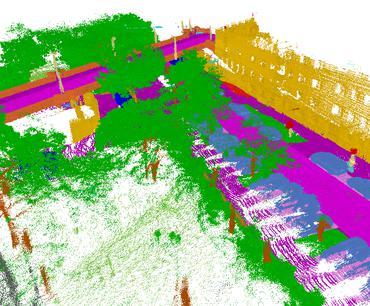
\includegraphics[width=0.7\textwidth]{images/semantickitti.jpg}
  \caption{SemanticKitti Frame: Each point has a color-coded class label.}
  \label{fig:semantickitti-frame}
\end{figure}

3D Semantic Segmentation assigns semantic class labels to each element of 3D data, usually a Point Cloud. It is not straightforward to apply 2D Semantic Segmentation techniques to 3D data for a number of reasons. One issue is that 3D data is sparse: every pixel in an image has useful information but the majority of space in a voxelized point cloud is completely empty. Another issue is the exponential growth of memory requirements and processing time required by adding another dimension. Finally, while camera imagery is ubiquitous and relatively easy to label, 3D data is more expensive to collect and more difficult to train.

\subsection{Datasets}
\label{sec:datasets}

Datasets are collections of raw point cloud data along with per-point hand-labeled "ground truth" datum. No dataset is perfectly representative of the world, so it's important to test algorithms against as diverse a set as possible. Unfortunately, most segmentation algorithms only test their performance against one or two of the most popular publicly available datasets. Thus one goal of this projct is to see how state of the art algorithms perform against other, possibly more challenging, dataset.

We consider the datasets listed in Table \ref{tab:datasets}:
\begin{enumerate}
  \item SemanticKitti \cite{semantickitti1,semantickitti2}: One of the first publicly available datasets, SemanticKitti is the de facto standard against which most algorithms test. This dataset features city driving in Germany with 28 semantic classes.
  \item nuScenes \cite{nuscenes}: This is the second most popular dataset available. It features complex city driving in Boston and Singapore, including driving in adverse weather conditions, with 32 semantic classes.
  \item Rellis3D \cite{rellis3d}: A product of collaboration between the Army Research Lab and Texas A\&M University, this dataset features 20 semantic classes in offroad conditions.
\end{enumerate}

\begin{figure}[htp]
  \centering
  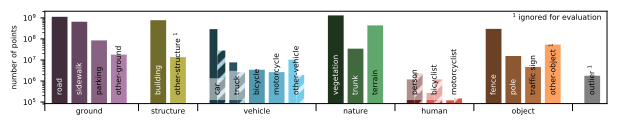
\includegraphics[width=0.7\textwidth]{images/semantic_kitti_label_distribution.png}
  \caption{SemanticKitti label distribution}
  \label{fig:semantickitti-label-distribution}
\end{figure}

\begin{figure}[htp]
  \centering
  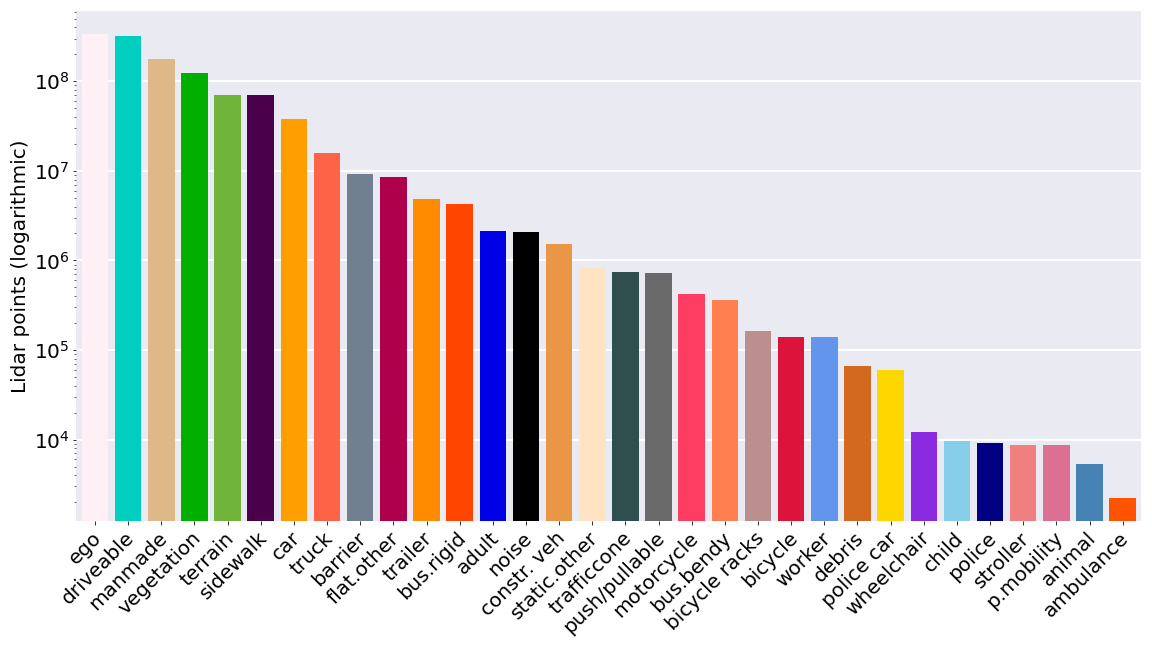
\includegraphics[width=0.7\textwidth]{images/nuscenes_label_set.png}
  \caption{nuScenes label distribution}
  \label{fig:nuscenes-label-set}
\end{figure}

\begin{figure}[htp]
  \centering
  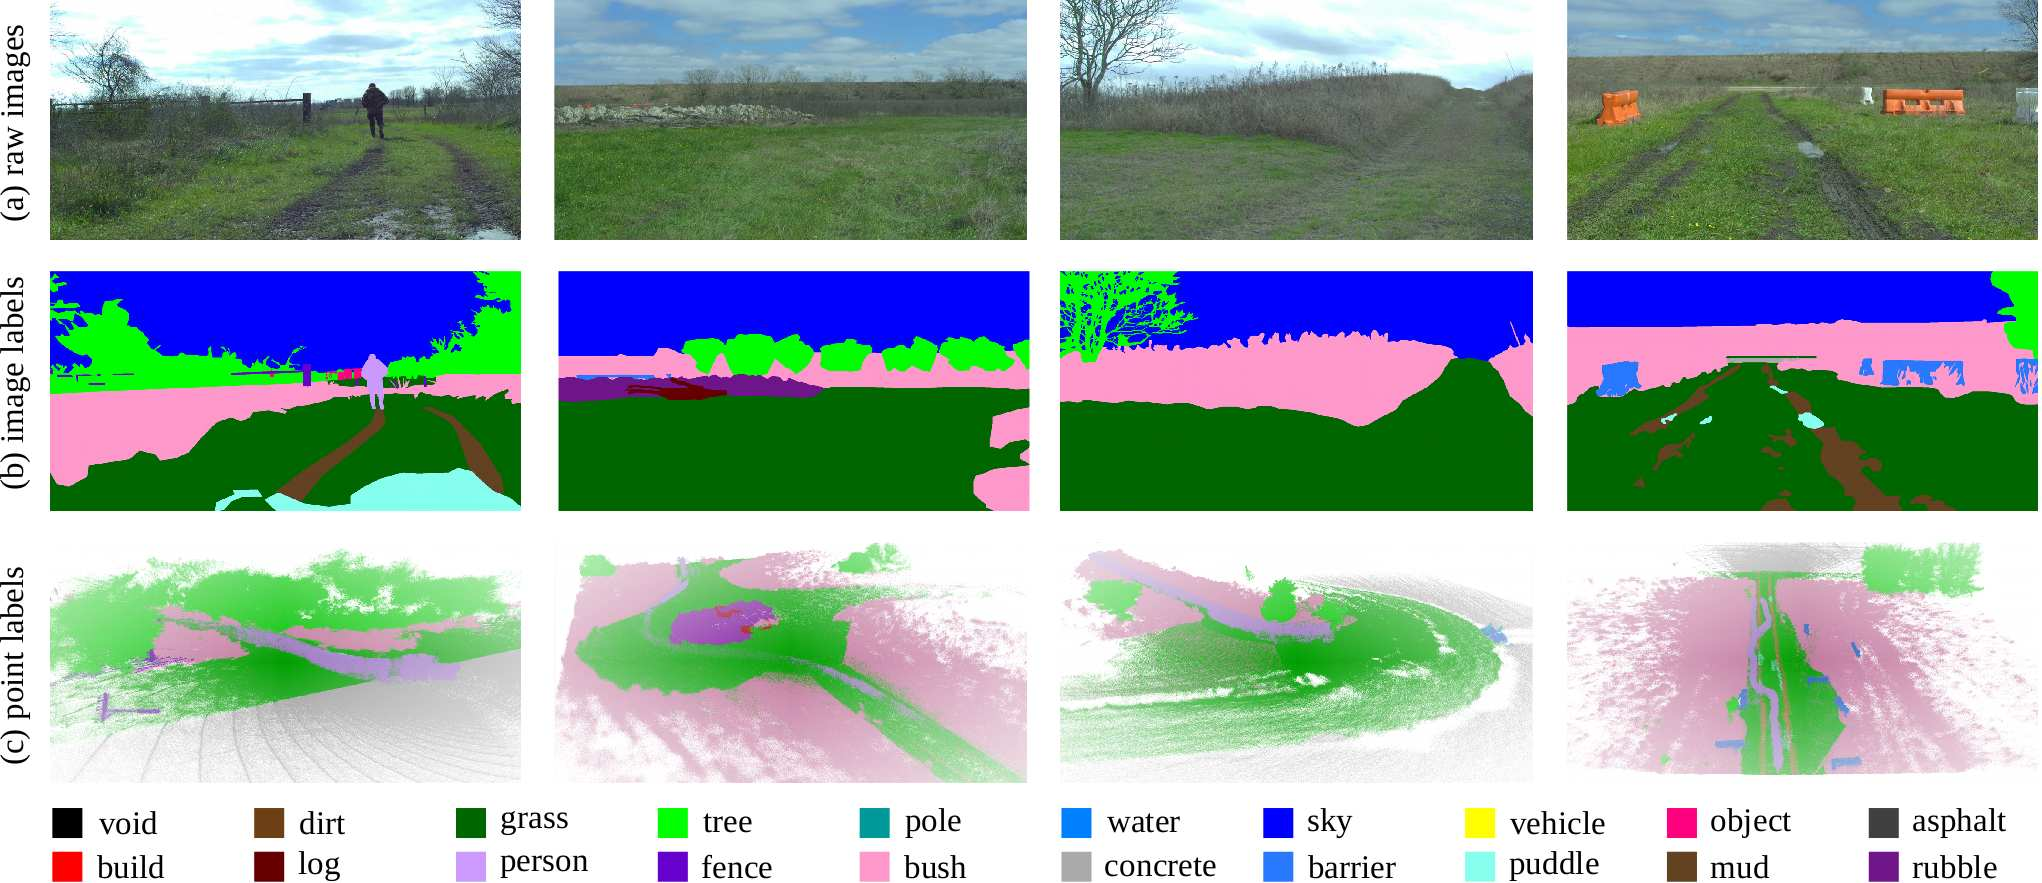
\includegraphics[width=0.7\textwidth]{images/rellis_label_suite.png}
  \caption{Rellis3D label distribution}
  \label{fig:rellis-labe-suite}
\end{figure}

\subsection{Segmenters}
\label{sec:segmenters}

There are many different approaches to the problem of 3D Semantic Segmentation \cite{deeplearningpcsurvey}. Some aim to get the best possible score for a given challenge using pure 3D data; others use multimodal fusion. Some are less focused on overall performance and instead attempt to make do with less data or less labeled data \cite{2dpass}. Some tackle the problem of sparsity with sparse convolution \cite{sparseconv}; others reject a voxelized representation in favor of pure point-based representations \cite{pointnet}. We selected the following from the leaderboards for the last few years.

\begin{enumerate}
  \item SalsaNext \cite{salsanext}: A range-image based approach which was released in 2020 and benchmarked against SemanticKitti.
  \item Cylinder3D \cite{cylinder3d}: A cylindrical voxelization scheme is used in conjunction with sparse convolution in this 2020 paper which topped the leaderboards for both nuScenes and SemanticKitti.
  \item 2DPASS \cite{2dpass}: A multimodal approach which augments the 3D information with imagery. Released in 2022, this approach tops the SemanticKitti challenge as of this writing.
  \item COARSE3D \cite{coarse3d}: An approach to training which tackles the problem of limited annotations - this method trains against a limited subset of ground truth annotations via pixel anchors.
\end{enumerate}

\begin{figure}[htp]
  \centering
  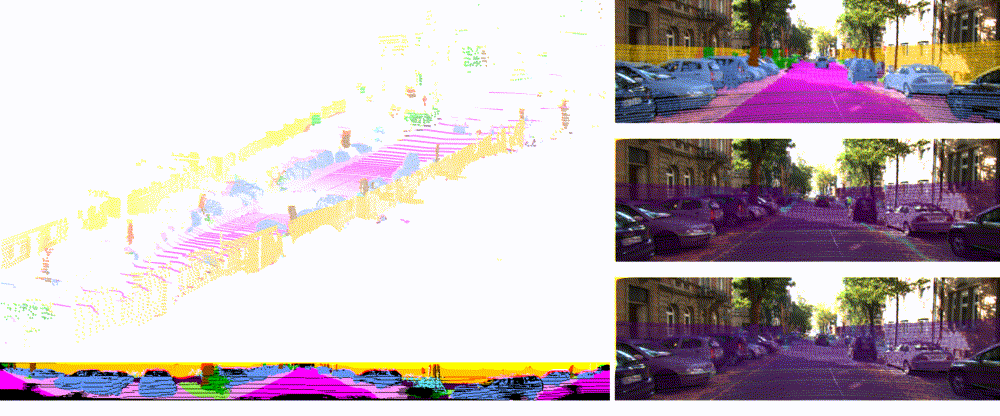
\includegraphics[width=0.7\textwidth]{images/salsanext_overview.png}
  \caption{SalsaNext overview}
  \label{fig:salsanext-overview}
\end{figure}

\begin{figure}[htp]
  \centering
  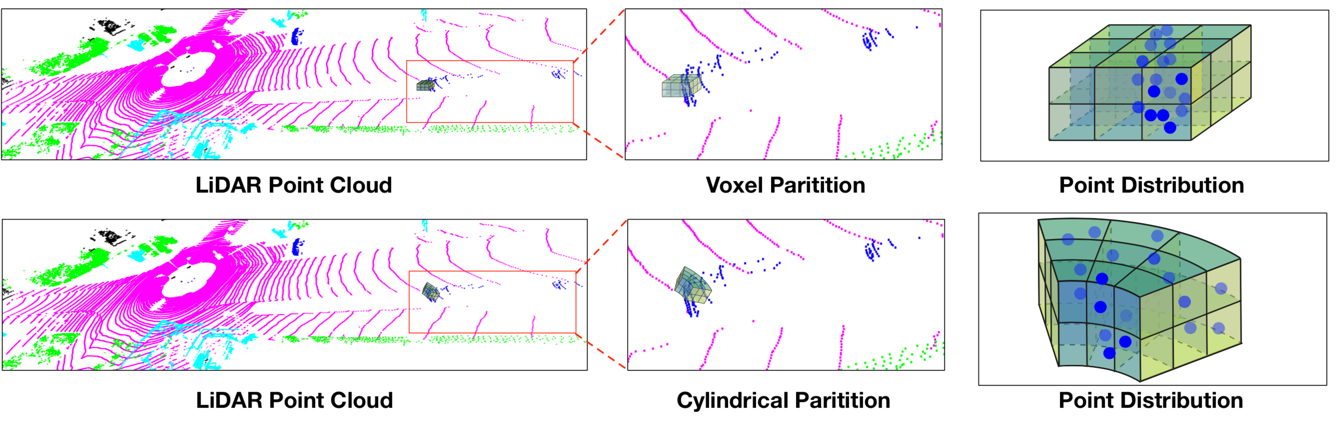
\includegraphics[width=0.7\textwidth]{images/cylinder3d_overview.png}
  \caption{Cylinder3D overview}
  \label{fig:cylinder3d-overview}
\end{figure}

\begin{figure}[htp]
  \centering
  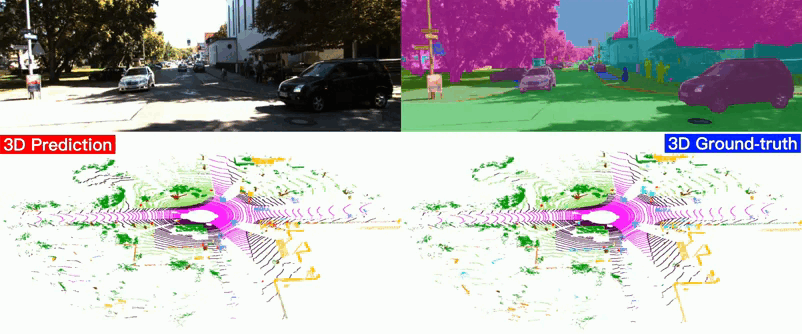
\includegraphics[width=0.7\textwidth]{images/2DPASS_overview.png}
  \caption{2DPASS overview}
  \label{fig:2dpass-overview}
\end{figure}

\begin{figure}[htp]
  \centering
  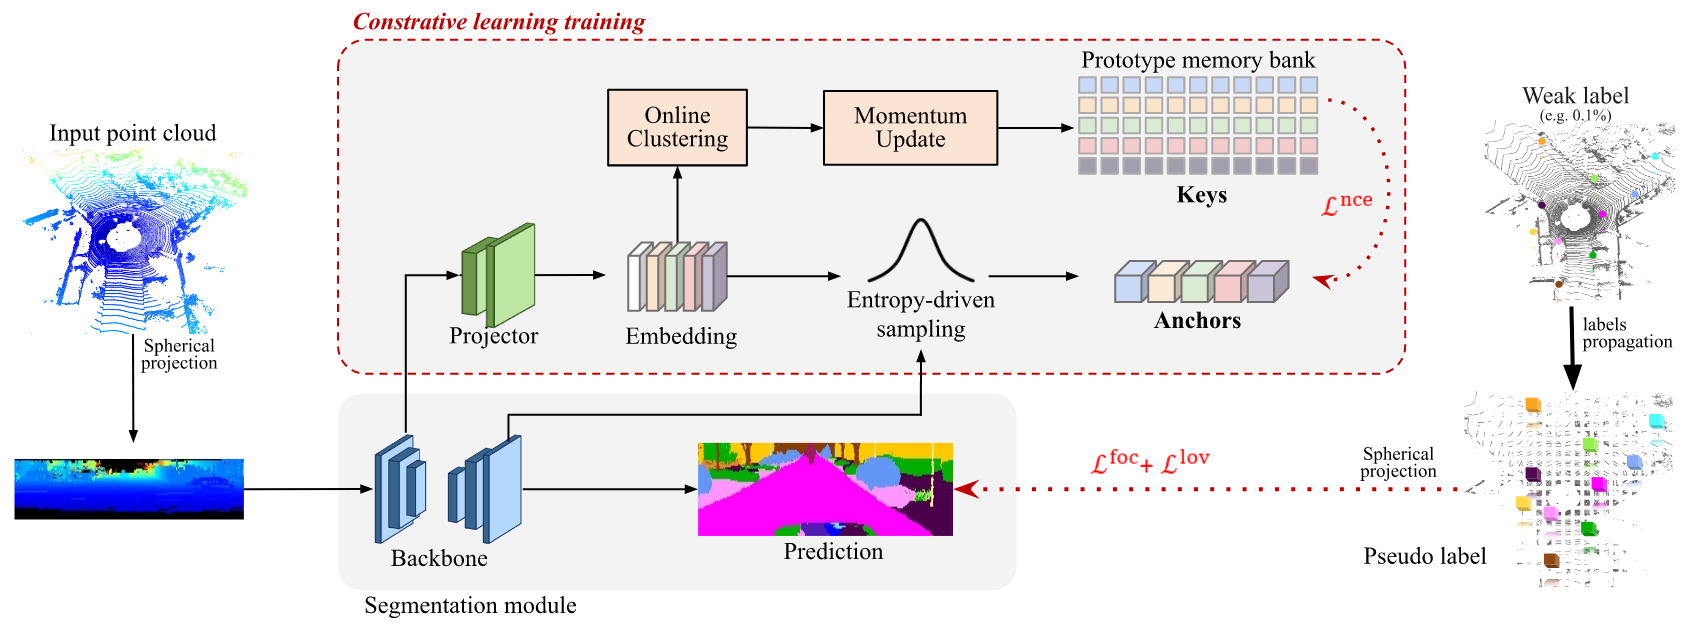
\includegraphics[width=0.7\textwidth]{images/coarse3d_overview.png}
  \caption{COARSE3D overview}
  \label{fig:coarse3d-overview}
\end{figure}

